\documentclass[tikz]{standalone}
\usepackage{amsmath}
\usepackage{pgfplots}
\pgfplotsset{compat=newest}
\usetikzlibrary{backgrounds}

\begin{document}
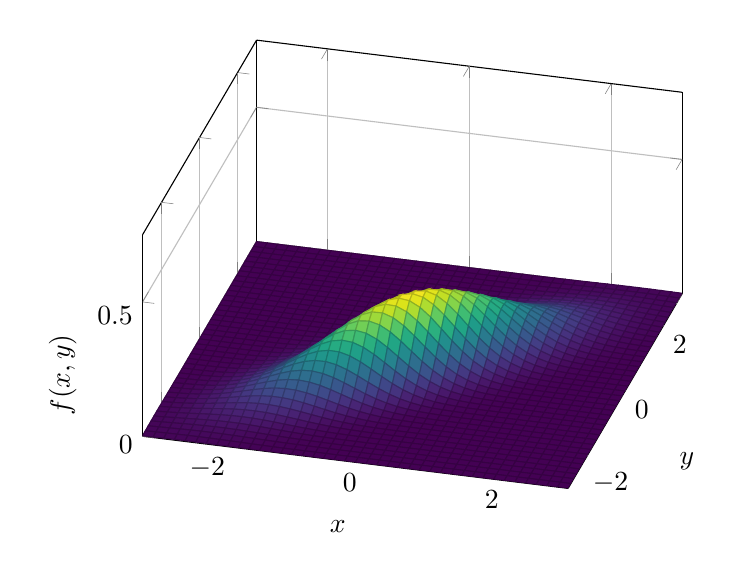
\begin{tikzpicture}[background rectangle/.style={fill=white}, show background rectangle,]

\begin{axis}[
    colormap/viridis,
    view={15}{45},
    enlargelimits=false,
    grid=major,
    domain=-3:3,
    y domain=-3:3,
    samples=41,
    zmin=0,
    zmax=0.75,
    xlabel=$x$,
    ylabel=$y$,
    zlabel={$f(x,y)$},
]
\addplot3 [surf] { 1 / (2*pi*1*1*sqrt(1-(0.8)^2)) * exp(-1/(2*(1-(0.8)^2)) * ((x^2 / 1^2) + (y^2 / 1^2) - 2*0.8*x*y/(1*1))) } ;
\end{axis}
\end{tikzpicture}
\end{document}
